% ============================================================
%  ROZDZIAŁ: Profilowanie badaczy
%  Wymagane pakiety: graphicx, booktabs, float, amsmath,
%                   caption, subcaption, hyperref, array
% ============================================================

\chapter{Profilowanie badaczy na podstawie ich działalności naukowej
         oraz analiza zachowań profili w~zależności od~zastosowanych
         podejść profilowania}

% ----------------------------------------------------------
\section{Zbiór danych}
\label{sec:dataset}
% ----------------------------------------------------------

Eksperymenty opisane w~niniejszym rozdziale przeprowadzono na~danych
dotyczących pracowników naukowych Wydziału Matematyki i~Informatyki
(WMIi) Uniwersytetu im.~Adama Mickiewicza w~Poznaniu.
Wydział ten skupia badaczy reprezentujących szerokie spektrum
dyscyplin: od~matematyki czystej (analiza funkcjonalna, kombinatoryka,
topologia) poprzez informatykę teoretyczną i~algorytmikę,
aż po~uczenie maszynowe, przetwarzanie języka naturalnego
i~grafikę komputerową.
Taka różnorodność tematyczna czyni zbiór szczególnie wartościowym
do~testowania metod profilowania semantycznego: dobry model powinien
zarówno wyraźnie separować naukowców z~odległych dziedzin,
jak i~blisko umieszczać tych o~zbieżnych zainteresowaniach.

\subsection{Źródła danych}

Profile naukowców (identyfikatory ORCID, afiliacje, imiona i~nazwiska)
pozyskano z~Portalu Badawczego UAM.
Publikacje pobrano za pomocą API serwisu OpenAlex~\cite{priem2022openalex} --
otwartego indeksu prac naukowych, który agreguje metadane
z~Crossref, PubMed, arXiv i~innych źródeł.
Dla każdego naukowca wysłano zapytanie filtrowane identyfikatorem
ORCID, co~zapewniło jednoznaczne przypisanie prac do~autorów.

\subsection{Statystyki zbioru}

Ostateczny zbiór danych obejmuje:
\begin{itemize}
    \item \textbf{164 naukowców} posiadających identyfikator ORCID,
    \item \textbf{3~440 publikacji} z~tytułem i~abstraktem w~języku angielskim,
    \item \textbf{57 unikalnych par współautorskich} wyodrębnionych spośród
          naukowców uwzględnionych w~zbiorze
          (średnia liczba wspólnych prac na~parę: 4{,}4).
\end{itemize}

Spośród 164 naukowców \textbf{107} posiada co~najmniej 3~publikacje
w~zbiorze (mediana: 20~prac, maksimum: 199~prac) i~tylko ta~podgrupa
brana jest pod uwagę w~eksperymentach wymagających minimalnego dorobku.
Rozkład liczby publikacji jest silnie prawostronnie skośny:
większość badaczy ma kilkanaście–kilkadziesiąt prac,
podczas gdy kilku profesorów z~długim stażem przekracza 100~pozycji.

\subsection{Filtrowanie i~ograniczenia}

Do~eksperymentów włączono wyłącznie publikacje posiadające zarówno
tytuł, jak i~abstrakt w~języku angielskim.
Takie ograniczenie wynika z~faktu, że~wszystkie testowane modele
embeddingowe zostały wytrenowane przede wszystkim na~anglojęzycznych
korpusach naukowych; włączenie polskojęzycznych tekstów
bez~specjalistycznego modelu wielojęzycznego prowadziłoby
do~nierównomiernej jakości reprezentacji.
Prace bez abstraktu (np.\ artykuły konferencyjne sprzed epoki
systematycznej archiwizacji) zostały pominięte.

Pary współautorskie są stosowane jako \emph{proxy} podobieństwa
semantycznego (zob.\ sekcja~\ref{sec:validation}): zakłada się,
że~naukowcy współpiszący razem artykuły reprezentują bliskie obszary
badawcze i~ich profile powinny być semantycznie zbliżone.
Ograniczeniem tego założenia jest fakt, że~współautorstwo może
wynikać z~przyczyn administracyjnych lub projektowych,
niekoniecznie ze~zbieżności zainteresowań naukowych.

% ----------------------------------------------------------
\section{Modele embeddingów}
\label{sec:models}
% ----------------------------------------------------------

\subsection{Charakterystyka modeli wykorzystanych podczas analizy}
\label{subsec:models_overview}

W~eksperymentach porównano sześć modeli transformerowych
do~generowania wektorowych reprezentacji tekstów (embeddingów).
Tabela~\ref{tab:models_full} zestawia ich podstawowe właściwości.

\begin{table}[H]
\centering
\caption{Modele embeddingowe użyte w~eksperymentach.}
\label{tab:models_full}
\begin{tabular}{llccp{3.2cm}}
\toprule
\textbf{Skrót} & \textbf{Identyfikator (HuggingFace)} & \textbf{Wymiar} & \textbf{Parametry} & \textbf{Domena / trening} \\
\midrule
SPECTER            & \texttt{allenai/specter}                        & 768 & 110M & Naukowy (cytowania) \\
MiniLM-L6          & \texttt{all-MiniLM-L6-v2}                       & 384 & 22M  & Ogólny (destylacja) \\
MiniLM-L12         & \texttt{all-MiniLM-L12-v2}                      & 384 & 33M  & Ogólny (destylacja) \\
MPNet-Base         & \texttt{all-mpnet-base-v2}                      & 768 & 110M & Ogólny (MPNet) \\
BGE-Small          & \texttt{BAAI/bge-small-en-v1.5}                 & 384 & 24M  & Retrieval (kontrastywny) \\
Multilingual-MiniLM & \texttt{paraphrase-multilingual-MiniLM-L12-v2} & 384 & 118M & Wielojęzyczny \\
\bottomrule
\end{tabular}
\end{table}

Wszystkie modele zostały użyte bez~dodatkowego dostrajania (\textit{out-of-the-box}),
co~odzwierciedla realistyczny scenariusz wdrożeniowy, w~którym kosztowny
fine-tuning nie jest dostępny.

\subsubsection{SPECTER}

SPECTER (\textit{Scientific Paper Embeddings using Citation-informed
TransformERs})~\cite{specter2020} to~model zaproponowany przez Cohana i~in.,
zbudowany na~bazie SciBERT~\cite{scibert2019} -- wariantu BERT
wstępnie wytrenowanego na~korpusie ponad miliona pełnotekstowych artykułów
naukowych z~bazy Semantic Scholar.
Kluczową innowacją SPECTER jest drugi etap treningu: model optymalizowany jest
funkcją straty \textit{triplet margin loss}
\begin{equation}
    \mathcal{L}(a,p,n) = \max\bigl(0,\;
        \|\mathbf{E}(a) - \mathbf{E}(p)\|^2 -
        \|\mathbf{E}(a) - \mathbf{E}(n)\|^2 + m\bigr),
\end{equation}
gdzie $a$ jest artykułem zakotwiczenia (\textit{anchor}),
$p$ -- artykułem cytowanym przez $a$ (pozytywny),
$n$ -- artykułem negatywnym dobranym losowo,
a~$m$ -- marginesem separacji.
Sygnałem nadzoru jest zatem istniejąca struktura grafu cytowań,
a~nie ręcznie nadane etykiety tematyczne.
Wynikowa przestrzeń embeddingów ma~wymiar 768;
reprezentacja dokumentu uzyskiwana jest przez wybranie wektora
tokenu \texttt{[CLS]} z~ostatniej warstwy transformerowej.

\subsubsection{MiniLM-L6 (\texttt{all-MiniLM-L6-v2})}

Model \texttt{all-MiniLM-L6-v2}~\cite{wang2020minilm} łączy dwa podejścia:
destylację wiedzy (\textit{knowledge distillation}) z~frameworkiem
Sentence-BERT~\cite{sbert2019}.
Architektura składa się z~6~warstw transformerowych
(zamiast 12 w~oryginalnym BERT) o~rozmiarze ukrytym 384,
co~redukuje liczbę parametrów do~ok.~22 milionów.
W~procesie destylacji uczeń minimalizuje rozbieżność Kullbacka--Leiblera
między macierzami uwagi nauczyciela i~ucznia:
\begin{equation}
    \mathcal{L}_{\mathrm{KD}} = \mathrm{KL}(A_{\mathrm{teacher}} \| A_{\mathrm{student}}),
\end{equation}
co~pozwala przenieść wiedzę o~strukturze uwagi, nie tylko o~wynikach końcowych.
Model trenowany jest następnie w~architekturze syjamskiej
na~ponad miliardzie par zdań z~różnorodnych korpusów ogólnych,
z~zastosowaniem funkcji straty \textit{Multiple Negatives Ranking Loss}.
Reprezentacja zdania uzyskiwana jest przez \textit{mean pooling}
-- uśrednianie wektorów wszystkich tokenów z~ostatniej warstwy.

\subsubsection{MiniLM-L12 (\texttt{all-MiniLM-L12-v2})}

\texttt{all-MiniLM-L12-v2} jest wariantem o~podwojonej głębokości
(12 warstw zamiast 6) przy tym samym rozmiarze ukrytym 384.
Procedura treningu jest analogiczna do~MiniLM-L6,
lecz większa pojemność modelu pozwala uchwycić subtelniejsze
relacje semantyczne kosztem nieco wyższego kosztu obliczeniowego.
W~eksperymentach oba warianty MiniLM zachowują się bardzo podobnie,
co~potwierdza dominację architektury i~danych treningowych
nad liczbą warstw w~tym przedziale parametrów.

\subsubsection{MPNet-Base (\texttt{all-mpnet-base-v2})}

MPNet~\cite{mpnet2020} to~architektura łącząca zalety BERT
(bierze pod uwagę zależności między wszystkimi tokenami)
i~XLNet (unika problemu rozbieżności między pre-treningiem
a~finetuningiem wynikającej z~maskowania).
Model \texttt{all-mpnet-base-v2} to~MPNet-Base
dostrojony do~generowania embeddingów zdaniowych na~szerokich,
różnorodnych korpusach podobieństwa semantycznego.
Wymiar wyjściowy wynosi 768; w~eksperymentach wymagających
porównywania z~modelami 384-wymiarowymi zastosowano
projekcję Johnsona--Lindenstraussa (zob.\ sekcja~\ref{subsec:jl}).

\subsubsection{BGE-Small (\texttt{BAAI/bge-small-en-v1.5})}

BGE-Small pochodzi z~rodziny modeli \textit{Beijing Academy of AI}
(BAAI)~\cite{bge2023}, zaprojektowanych z~myślą o~efektywnym
wyszukiwaniu informacji (\textit{retrieval}).
Model wytrenowany jest metodą uczenia kontrastywnego
z~trudnymi negatywami (\textit{hard negative mining}):
dla każdego przykładu pozytywnego dobierane są pary negatywne,
które są semantycznie bliskie, ale nie są odpowiedziami na~zapytanie.
Taka procedura wymusza tworzenie zwartych, tematycznie skupionych
reprezentacji -- właściwość ta~okazuje się kluczowa
dla szybkiej stabilizacji profilu naukowca
(zob.\ sekcja~\ref{sec:stability}).
Pomimo małych rozmiarów (384 wymiary, ok.~24M parametrów)
model osiąga wyniki porównywalne z~modelami wielokrotnie większymi.

\subsubsection{Multilingual-MiniLM (\texttt{paraphrase-multilingual-MiniLM-L12-v2})}

Model wielojęzyczny oparty na~architekturze MiniLM-L12,
dostrojony na~parach parafraz w~ponad 50~językach.
Włączony do~porównania jako punkt odniesienia dla scenariusza,
w~którym część publikacji mogłaby być dostępna w~językach innych
niż angielski (np.\ polskie monografie lub artykuły konferencyjne).
Jak wykazują eksperymenty, model ten wykazuje największą
rozbieżność w~stosunku do~pozostałych modeli anglojęzycznych,
co~prawdopodobnie wynika z~kompromisu między jakością
reprezentacji a~wielojęzycznym zakresem treningu.

\subsection{Projekcja Johnson--Lindenstraussa}
\label{subsec:jl}

Modele SPECTER i~MPNet-Base generują wektory o~wymiarze 768,
podczas gdy pozostałe cztery modele produkują wektory 384-wymiarowe.
Aby umożliwić bezpośrednie porównania i~konkatenacje embeddingów,
wektory 768-wymiarowe redukowano do~384 wymiarów za~pomocą
\emph{losowej projekcji liniowej}:
\begin{equation}
    \mathbf{e}' = \frac{1}{\sqrt{384}}\,\mathbf{e}\,\mathbf{P},
    \qquad \mathbf{P} \in \mathbb{R}^{768 \times 384},\;
    P_{ij} \sim \mathcal{N}(0,1),
    \label{eq:jl_proj}
\end{equation}
po~czym $\mathbf{e}'$ normalizowano do~normy jednostkowej $L_2$.
Podejście to~uzasadnia lemat Johnsona--Lindenstraussa~\cite{jl1984},
który gwarantuje, że~losowa projekcja z~wysokowymiarowej przestrzeni
do~przestrzeni o~wymiarze $k \geq \frac{8 \ln n}{\varepsilon^2}$
zachowuje parami odległości euklidesowe ze~zniekształceniem
co~najwyżej $(1 \pm \varepsilon)$ z~wysokim prawdopodobieństwem.
Macierz $\mathbf{P}$ jest deterministyczna (ustalono stałe ziarno
losowości), dzięki czemu wyniki są w~pełni powtarzalne.

% ----------------------------------------------------------
\section{Podejścia do~budowania profilu badacza}
\label{sec:approaches}
% ----------------------------------------------------------

\subsection{Reprezentacja centroidem}
\label{subsec:centroid}

Profil embeddingowy naukowca zdefiniowano jako \emph{centroid} --
średnią arytmetyczną wektorów embeddingowych jego indywidualnych
publikacji:
\begin{equation}
    \mathbf{c}_S = \frac{1}{|S|} \sum_{i \in S} \mathbf{e}_i,
    \label{eq:centroid_def}
\end{equation}
gdzie $\mathbf{e}_i \in \mathbb{R}^d$ jest embeddingiem $i$-tej pracy,
a~$S$ -- zbiorem prac naukowca (lub wybranym podzbiorem).

Reprezentacja centroidem posiada kilka kluczowych zalet praktycznych.
Po~pierwsze, \textbf{rozmiar profilu jest stały} niezależnie od~liczby
publikacji -- nie rośnie wraz z~dorobkiem autora, co~jest niezbędne
dla skalowalności systemu rekomendacji.
Po~drugie, \textbf{profil jest łatwo aktualizowalny inkrementalnie}:
dodanie nowej pracy wymaga jedynie aktualizacji centroidu
$\mathbf{c}_{S \cup \{j\}} = \frac{|S| \cdot \mathbf{c}_S + \mathbf{e}_j}{|S|+1}$,
bez ponownego przeliczania całego profilu.
Po~trzecie, centroid posiada interpretację geometryczną jako punkt
najlepiej reprezentujący chmurę wektorów publikacji w~sensie
minimalizacji sumarycznej odległości euklidesowej.

Alternatywą jest konkatenacja wszystkich tekstów publikacji
w~jeden długi dokument i~zakodowanie go jako jednego wektora.
Podejście to~zastosowano w~fazie wstępnej eksperymentów
(zob.\ sekcja~\ref{subsec:validation_coauthor}),
lecz ma~ono istotną wadę: dla naukowców z~dużym dorobkiem
łączny tekst przekracza okno kontekstowe modeli
(typowo 256--512 tokenów), co~prowadzi do~obcinania informacji.

\subsection{Embeddingi tytułów prac}
\label{subsec:titles}

Pierwszą i~najskromniejszą pod względem informacyjnym reprezentacją
jest embedding samego tytułu publikacji.
Tytuł stanowi zwięzłą deklarację tematu pracy, pozbawioną
szczegółów metodycznych ani wyników.
Zalety tego podejścia to~universalność (praktycznie każda publikacja
ma tytuł) i~odporność na~braki w~metadanych.

W~eksperymencie porównawczym (sekcja~\ref{sec:validation})
embeddingi tytułów wykazały zaskakująco dobrą zdolność
do~separowania grup tematycznych.
Wynika to~z~faktu, że~słownictwo tytułów naukowych jest
silnie specjalistyczne: słowa kluczowe dziedziny pojawiają się
już w~tytule, co~umożliwia modelowi poprawne wnioskowanie
o~temacie nawet bez treści.

\subsection{Embeddingi abstraktów prac}
\label{subsec:abstracts}

Abstrakt dostarcza znacznie więcej informacji niż sam tytuł:
opisuje motywację, zastosowaną metodę, dane i~główne wyniki.
Embeddingi abstraktów są zatem bogatszą reprezentacją pracy,
choć kosztem wyższego czasu przetwarzania i~konieczności
dostępności abstraktu w~metadanych.

Eksperyment ablacyjny wykazał, że~włączenie abstraktów powoduje
spójne przesunięcia pozycji naukowców w~przestrzeni PCA:
badacze z~pokrewnych dziedzin przemieszczają się w~podobnych
kierunkach, co~świadczy o~tym, że~abstrakty wnoszą
semantycznie spójną informację, a~nie szum~\cite{ic_report}.

W~eksperymencie porównawczym (sekcja~\ref{sec:validation})
konfiguracje oparte na~abstraktach i~na~tytułach wykazały
umiarkowaną zgodność co~do~rankingu sąsiadów
(Jaccard $\approx 0{,}70$ dla tego samego modelu,
różne typy tekstu), co~sugeruje, że~obydwa typy tekstu
niosą uzupełniającą, lecz nie identyczną informację.

\subsection{Embeddingi N-gramów zdań z~abstraktu (podejście wstępne)}
\label{subsec:ngrams}

W~fazie eksploracyjnej prototypowano alternatywną metodę
budowania reprezentacji: abstrakt dzielono na~zdania,
generowano wszystkie okna N-gramowe (tj.\ ciągi kolejnych zdań)
z~przesunięciem o~jedno zdanie, embeddowano każde okno osobno,
a~następnie uśredniano wynikowe wektory.
Celem było uchwycenie lokalnych kontekstów semantycznych
zawartych w~kolejnych akapitach abstraktu.

Podejście to~zostało zidentyfikowane jako obiecujące koncepcyjnie,
lecz w~toku eksperymentów nie wykazało jednoznacznej przewagi
nad prostym embeddingiem całego abstraktu, przy znacznie wyższym
koszcie obliczeniowym (wielokrotne wywołania modelu na~dokument).
Z~tego powodu metoda N-gramów zdaniowych nie była stosowana
w~dalszych eksperymentach i~pozostaje kierunkiem wartym
zbadania w~przyszłości.

\subsection{Konkatenacja embeddingów z~różnych modeli}
\label{subsec:concat}

Motywacją do~konkatenacji embeddingów dwóch różnych modeli jest hipoteza,
że~różne modele mogą kodować uzupełniające sygnały semantyczne:
SPECTER opiera się na~strukturze cytowań, modele ogólne --
na~szerokim rozumieniu języka naturalnego.
Połączenie ich reprezentacji mogłoby dać profil bogatszy
niż każdy z~modeli osobno.

Technicznie, dla naukowca $a$ jego profil konkatenowany definiuje się jako:
\begin{equation}
    \mathbf{c}^{\oplus}_{a} =
    \bigl[\,\mathbf{c}^{(M_1)}_{a} \;\|\; \mathbf{c}^{(M_2)}_{a}\,\bigr]
    \;\in\; \mathbb{R}^{384+384},
\end{equation}
gdzie $\mathbf{c}^{(M_i)}_{a}$ jest centroidem modelu $M_i$
(po~ewentualnej projekcji do~wymiaru 384),
a~$\|$ oznacza konkatenację wektorów.
Podobieństwo między profilami dwóch naukowców obliczano
jako kosinusowe na~wektorach 768-wymiarowych.

Eksperyment zbadał kilkanaście par modeli,
m.in.\ MiniLM-L6~$\oplus$~SPECTER,
MiniLM-L6~$\oplus$~BGE-Small,
MiniLM-L6~$\oplus$~MPNet-Base.
Wizualizacje PCA i~macierze Jaccarda sąsiadów wskazują,
że~konkatenacja przesuwa ``mapę'' naukowców w~sposób,
który zależy od~wkładu obu modeli składowych.
Pełna, ilościowa ocena tej metody względem najlepszego
pojedynczego modelu pozostaje przedmiotem dalszych badań.

% ----------------------------------------------------------
\section{Metody walidacji profili badaczy}
\label{sec:validation}
% ----------------------------------------------------------

\subsection{Walidacja hipotezy bliskości współautorów}
\label{subsec:validation_coauthor}

Fundamentalnym pytaniem jest, czy~embeddingi publikacji
w~ogóle skutecznie reprezentują podobieństwo naukowe.
Do~weryfikacji tej hipotezy zastosowano test bliskości współautorów:
\textbf{jeśli dwoje naukowców współtworzyło co~najmniej jedną publikację,
ich profile powinny być semantycznie bliższe niż profile
losowo dobranych par}.

\subsubsection{Metodologia testu}

Dla każdego autora $a$ skonstruowano jego profil jako wektor
$\mathbf{E}(a)$ -- w~tej fazie przez konkatenację tytułów i~abstraktów
wszystkich prac w~jeden ciąg i~zakodowanie go~jako jeden wektor
(bez~uśredniania).
Podobieństwo między dwoma autorami zdefiniowano jako:
\begin{equation}
    \mathrm{sim}(a,b)
    = \frac{\mathbf{E}(a)\cdot\mathbf{E}(b)}
           {\|\mathbf{E}(a)\|\,\|\mathbf{E}(b)\|}.
\end{equation}
Obliczono podobieństwo dla:
\begin{itemize}
    \item 57~par współautorskich (ground truth: podobni),
    \item 1~000~losowo dobranych par spośród pozostałych
          (rozkład referencyjny).
\end{itemize}
Jako miarę separacji zastosowano jednostronny test Manna--Whitneya U
(hipoteza alternatywna: współautorzy $>$ losowe pary)
oraz rozmiar efektu $d$ Cohena~\cite{cohen1988}.

\subsubsection{Wyniki}

\begin{table}[H]
\centering
\caption{Wyniki testu bliskości współautorów dla dwóch modeli.}
\label{tab:coauthor_test}
\begin{tabular}{lcccccc}
\toprule
\textbf{Model} &
\textbf{Śr. sim.} & \textbf{Śr. sim.} & \textbf{Różnica} &
\textbf{$d$ Cohena} & \textbf{$p$-wartość} \\
& \textbf{(współaut.)} & \textbf{(losowe)} & & & \\
\midrule
SPECTER   & 0{,}787 & 0{,}624 & +0{,}163 & 1{,}51 & $1{,}82 \times 10^{-17}$ \\
MiniLM-L6 & 0{,}419 & 0{,}109 & +0{,}310 & 2{,}19 & $9{,}11 \times 10^{-20}$ \\
\bottomrule
\end{tabular}
\end{table}

Wyniki potwierdzają centralną hipotezę projektu SARA:
obydwa modele osiągają statystycznie wysoce istotną separację
($p < 10^{-16}$, rozmiar efektu $d \gg 0{,}8$),
co~oznacza, że~embeddingi tekstowe skutecznie kodują podobieństwo
naukowe bez~ręcznej taksonomii ani słów kluczowych.

Nieintuicyjnym wynikiem jest \textbf{wyraźna przewaga MiniLM-L6
nad SPECTER} ($d = 2{,}19$ vs $d = 1{,}51$) mimo~że SPECTER
trenowany był specjalnie na~tekstach naukowych.
Wyjaśnienia dostarcza geometria przestrzeni embeddingów:
SPECTER charakteryzuje się efektem \emph{kompresji} --
nawet losowe pary autorów osiągają średnie podobieństwo~$0{,}624$,
co~pozostawia mało miejsca na~dyskryminację.
MiniLM-L6 rozciąga swoją przestrzeń szerzej (losowe pary: $0{,}109$),
przez co~różnica między parami podobnymi a~losowymi jest prawie
dwukrotnie większa w~wartościach bezwzględnych.

Korelacja Pearsona między pełnymi macierzami podobieństwa
obu modeli wynosi $r = 0{,}729$ ($p \approx 0$),
co~świadczy o~umiarkowanie silnej, ale~nie pełnej zgodności:
modele zgadzają się co~do~ogólnej struktury podobieństwa,
lecz różnią się w~szczegółach rankingów.

\subsection{Podobieństwo Jaccarda dla zbiorów sąsiadów}
\label{subsec:jaccard}

Po~walidacji samego podejścia kolejnym krokiem jest porównanie,
\textbf{jak spójne rankingi sąsiadów generują różne konfiguracje
modeli i~typów tekstu}.
Dla każdego z~107 naukowców wyznaczono listę $K$ najbliższych sąsiadów
(top-$K$ NN) na~podstawie kosinusowego podobieństwa centroidów.
Pairwise overlap dwóch konfiguracji $A$ i~$B$ dla naukowca $s$
definiuje się jako:
\begin{equation}
    J_s(A, B) = \frac{|\mathrm{NN}_K^A(s) \cap \mathrm{NN}_K^B(s)|}
                     {|\mathrm{NN}_K^A(s) \cup \mathrm{NN}_K^B(s)|},
\end{equation}
a~wynikowa miara to~średnia po~wszystkich naukowcach:
$\bar{J}(A,B) = \frac{1}{N}\sum_s J_s(A,B)$.

\subsubsection{Wyniki}

Porównano wszystkie 67~unikalnych par spośród 12~konfiguracji
(6~modeli $\times$ 2~typy tekstu: tytuł / abstrakt).
Tabela~\ref{tab:jaccard_top} prezentuje ekstrema.

\begin{table}[H]
\centering
\caption{Wybrane pary konfiguracji według średniego podobieństwa Jaccarda.}
\label{tab:jaccard_top}
\begin{tabular}{llcc}
\toprule
\textbf{Konfiguracja A} & \textbf{Konfiguracja B} &
\textbf{Śr. Jaccard} & \textbf{Śr. overlap} \\
\midrule
MiniLM-L6\_abstract   & MiniLM-L12\_abstract    & 0{,}792 & 0{,}873 \\
MiniLM-L6\_title      & MiniLM-L12\_title       & 0{,}790 & 0{,}872 \\
MiniLM-L6\_title      & MPNet-Base\_title       & 0{,}762 & 0{,}853 \\
\midrule
Specter\_title        & Multilingual-MiniLM\_title  & 0{,}454 & 0{,}602 \\
Specter\_abstract     & Multilingual-MiniLM\_title  & 0{,}440 & 0{,}589 \\
\bottomrule
\end{tabular}
\end{table}

Wyniki wskazują na~\textbf{dwa klastry modeli}:
\begin{itemize}
    \item \textbf{Klaster spójny:} MiniLM-L6, MiniLM-L12, MPNet-Base
    -- modele te~generują bardzo zbliżone rankingi sąsiadów
    (Jaccard $0{,}76$--$0{,}79$), niezależnie od~tego,
    czy~embeddowany jest tytuł, czy~abstrakt.
    \item \textbf{Modele odmienne:} SPECTER i~Multilingual-MiniLM
    -- wykazują najniższą zgodność z~pozostałymi
    oraz między sobą (Jaccard $\approx 0{,}44$--$0{,}60$).
\end{itemize}

Pytanie o~to, \emph{który} model wskazuje ``właściwych'' sąsiadów,
pozostaje otwarte wobec braku złotego standardu.
Zjawisko rozbieżności sugeruje jednak, że~SPECTER i~Multilingual-MiniLM
kodują inny wymiar podobieństwa niż modele ogólne,
co~stanowi argument za~dalszym badaniem konkatenacji embeddingów
(sekcja~\ref{subsec:concat}).

\subsection{Podobieństwo cosinusowe centroidu cząstkowego do~pełnego}
\label{subsec:cosine_stability}

Miara ta~jest stosowana w~eksperymentach nad stabilnością profilu
(sekcja~\ref{sec:stability}).
Dla naukowca posiadającego $n$ prac, losowo wybierany jest podzbiór
$S \subset \{1,\ldots,n\}$, $|S|=k$.
Miarą wierności centroidu cząstkowego $\mathbf{c}_S$
względem centroidu pełnego $\mathbf{c}_{\mathrm{all}}$ jest:
\begin{equation}
    \mathrm{stab}(k) =
    \mathrm{sim}(\mathbf{c}_S, \mathbf{c}_{\mathrm{all}})
    = \frac{\mathbf{c}_S \cdot \mathbf{c}_{\mathrm{all}}}
           {\|\mathbf{c}_S\|\,\|\mathbf{c}_{\mathrm{all}}\|}.
\end{equation}
Wartość $\mathrm{stab}(k) \to 1$ gdy $k \to n$
(centroid podzbioru zbiega do~centroidu pełnego).
Za~progi praktycznej stosowalności przyjęto
$\mathrm{stab} \geq 0{,}95$ (akceptowalne odchylenie)
i~$\mathrm{stab} \geq 0{,}99$ (wysoka wierność).

% ----------------------------------------------------------
\section{Czynniki wpływające na~stabilność profilu}
\label{sec:stability}
% ----------------------------------------------------------

Kluczowym pytaniem praktycznym jest: \textbf{ile publikacji potrzeba,
by~profil embeddingowy był wiarygodną reprezentacją dorobku naukowca?}
Odpowiedź ma~bezpośrednie znaczenie dla jakości systemu rekomendacji --
naukowcy z~małym dorobkiem (doktoranci, asystenci)
nie powinni być dyskwalifikowani, jeśli kilka prac wystarczy
do~uformowania stabilnego profilu.

% ============================================================
%  SEKCJA: Analiza stabilności centroidu naukowca
%  Wklej do dokumentu głównego; wykresy umieść w katalogu figures/
%  Wymagane pakiety: graphicx, booktabs, float, amsmath, caption, subcaption
% ============================================================

\section{Analiza stabilności centroidu profilu naukowca}
\label{sec:centroid-stability}

% ----------------------------------------------------------
\subsection{Motywacja}
% ----------------------------------------------------------

Profil embeddingowy naukowca wyznaczamy jako \emph{centroid} -- średnią wektorów
reprezentujących poszczególne publikacje:
\begin{equation}
    \mathbf{c}_S \;=\; \frac{1}{|S|} \sum_{i \in S} \mathbf{e}_i,
    \label{eq:centroid}
\end{equation}
gdzie $\mathbf{e}_i \in \mathbb{R}^d$ jest embeddingiem $i$-tej pracy
i~$S$ -- wybranym podzbiorem prac naukowca.
Kluczowym pytaniem praktycznym jest: \textbf{ile publikacji potrzeba,
by centroid $\mathbf{c}_S$ był wiarygodną aproksymacją centroidu
pełnego $\mathbf{c}_\text{all}$, wyznaczonego ze wszystkich dostępnych prac?}
Odpowiedź ma bezpośrednie znaczenie dla jakości systemu rekomendacji --
naukowcy z~małym dorobkiem nie powinni być z~góry dyskwalifikowani,
jeśli już kilka prac wystarcza do uformowania stabilnego profilu.

% ----------------------------------------------------------
\subsection{Dane i metodologia}
% ----------------------------------------------------------

\subsubsection{Zbiór danych i modele embeddingowe}

Eksperymenty przeprowadzono na zbiorze $N = 164$ pracowników naukowych
Uniwersytetu im.~Adama Mickiewicza w~Poznaniu.
Dla każdej ze~$3\,440$ zidentyfikowanych publikacji wyznaczono embedding
\emph{tytułu} przy użyciu sześciu modeli transformerowych (Tabela~\ref{tab:models}).

\begin{table}[H]
\centering
\caption{Modele embeddingowe użyte w~eksperymencie.}
\label{tab:models}
\begin{tabular}{llcc}
\toprule
\textbf{Skrót} & \textbf{Identyfikator modelu} & \textbf{Wymiar} & \textbf{Domena} \\
\midrule
MiniLM-L6          & \texttt{all-MiniLM-L6-v2}                          & 384 & ogólny \\
Specter             & \texttt{allenai/specter}                             & 768 & naukowy \\
MPNet-Base          & \texttt{all-mpnet-base-v2}                          & 768 & ogólny \\
Multilingual-MiniLM & \texttt{paraphrase-multilingual-MiniLM-L12-v2}     & 384 & wielojęz. \\
MiniLM-L12          & \texttt{all-MiniLM-L12-v2}                         & 384 & ogólny \\
BGE-Small           & \texttt{BAAI/bge-small-en-v1.5}                    & 384 & retrieval \\
\bottomrule
\end{tabular}
\end{table}

Modele o~wymiarze $768$ (Specter, MPNet-Base) sprowadzono do wymiaru $384$
za~pomocą \emph{losowej projekcji liniowej} opartej na~lemacie
Johnsona--Lindenstraussa~\cite{johnson1984extensions}.
Dla wektora $\mathbf{e} \in \mathbb{R}^{768}$ projekcja przyjmuje postać:
\begin{equation}
    \mathbf{e}' \;=\; \frac{1}{\sqrt{384}}\,\mathbf{e}\,\mathbf{P},
    \qquad \mathbf{P} \in \mathbb{R}^{768 \times 384},\; P_{ij} \sim \mathcal{N}(0,1),
    \label{eq:jl}
\end{equation}
po~czym $\mathbf{e}'$ normalizowano do~normy jednostkowej~$L_2$.
Macierz $\mathbf{P}$ jest deterministyczna (ustalono ziarno losowości),
dzięki czemu wyniki są w~pełni powtarzalne.
Liniowość projekcji gwarantuje, że
$\operatorname{resize}(\bar{\mathbf{e}}) = \overline{\operatorname{resize}(\mathbf{e})}$,
tzn.\ centroid z~przeskalowanych wektorów jest równoważny przeskalowaniu
gotowego centroidu.

\subsubsection{Miara stabilności}

Jako miarę zbieżności centroidu podzbioru do centroidu pełnego stosujemy
\textbf{podobieństwo cosinusowe}:
\begin{equation}
    \mathrm{sim}(\mathbf{c}_S,\,\mathbf{c}_\text{all})
    \;=\;
    \frac{\mathbf{c}_S \cdot \mathbf{c}_\text{all}}
         {\|\mathbf{c}_S\|\;\|\mathbf{c}_\text{all}\|}.
    \label{eq:cosine}
\end{equation}
Wartość~1 oznacza identyczny kierunek w~przestrzeni wektorowej
(profil zbudowany z~podzbioru jest identyczny z~profilem pełnym);
wartości bliskie~0 wskazują na~brak korelacji między centroidami.
Za progi praktycznej stosowalności przyjęto $\mathrm{sim} \geq 0{,}95$
(dopuszczalne odchylenie) oraz $\mathrm{sim} \geq 0{,}99$ (wysoka wierność).

\subsubsection{Schemat eksperymentu}

Przeprowadzono trzy eksperymenty:

\begin{enumerate}
    \item \textbf{Eksperyment pilotażowy (Exp1).}
    Jeden naukowiec -- prof.~UAM dr~hab.~Tomasz~Górecki
    (ORCID: \texttt{0000-0002-9969-5257}, $n_\text{all} = 114$ prac) --
    jako reprezentatywny przypadek naukowca o~szerokim i~interdyscyplinarnym dorobku
    (statystyka funkcjonalna, klasyfikacja szeregów czasowych, chemometria).
    Dla rozmiarów próbki $k \in \{3, 5, 10\}$ wygenerowano po~3 losowe podzbiory;
    dodatkowo wyznaczono centroid ze~wszystkich 114~prac.

    \item \textbf{Eksperyment rozszerzony -- gęste próbkowanie (Exp2).}
    Dla tego samego naukowca wygenerowano po~$K = 300$ unikalnych losowych
    podzbiorów dla każdego rozmiaru $k \in \{3, 5, 10, 20, 30, 50, 100\}$
    (rozmiar~$k=150$ pominięto, ponieważ naukowiec ma jedynie 114~prac).
    Łącznie $300 \times 7 + 1 = 2\,101$ centroidów na~model.
    Unikalne podzbiory gwarantowano przez śledzenie zbioru wygenerowanych
    zestawów (struktura \texttt{frozenset}); powtórzenia między różnymi
    rozmiarami~$k$ były dozwolone.

    \item \textbf{Eksperyment zbiorczy -- 107~naukowców (Exp3).}
    Eksperyment rozszerzono na~wszystkich 107~naukowców UAM posiadających
    co~najmniej 3~prace w~zbiorze danych (mediana: 20~prac, max: 199~prac).
    Dla każdego naukowca, modelu i~rozmiaru $k \in \{3, 5, 10, 20, 50, 100\}$
    wygenerowano po~$N = 10$ losowych podzbiorów.
    Wyniki uśredniono po~naukowcach.
\end{enumerate}

% ----------------------------------------------------------
\subsection{Wyniki}
% ----------------------------------------------------------

\subsubsection{Eksperyment pilotażowy -- wizualizacja PCA}

Rysunek~\ref{fig:pca_centroid} przedstawia centroidy prof.~Góreckiego
zrzutowane na~płaszczyznę dwóch głównych składowych (PCA na~znormalizowanych
$L_2$ wektorach centroidów).
Każdy punkt odpowiada centroidowi zbudowanemu z~$k \in \{3, 5, 10\}$~losowych prac;
gwiazdka oznacza centroid pełny (wszystkie 114~prac).

\begin{figure}[H]
    \centering
    
\includegraphics[width=\textwidth]{pubs_num_stability/pca_centroid_stability.png}
    \caption{Wizualizacja PCA centroidów prof.~UAM dr~hab.~Tomasza Góreckiego
    dla sześciu modeli embeddingowych (3~powtórzenia na~rozmiar próbki).
    Czerwone punkty ($k=3$), żółte ($k=5$), niebieskie ($k=10$),
    zielona gwiazdka -- centroid ze~wszystkich 114~prac.
    Skupienie punktów wokół gwiazdki oznacza wysoką stabilność centroidu.}
    \label{fig:pca_centroid}
\end{figure}

Widoczna jest wyraźna różnica między modelami.
Dla \textbf{Spectera} i~\textbf{BGE-Small} wszystkie 9~centroidów
(niezależnie od~$k$) skupia się ściśle wokół centroidu pełnego --
nawet przy zaledwie 3~pracach centroid jest zbliżony do reprezentacji
opartej na~całym dorobku.
Dla modeli ogólnych (MiniLM-L6, MiniLM-L12, MPNet-Base,
Multilingual-MiniLM) centroidy przy $k=3$ są rozrzucone daleko
od~centroidu pełnego, a~dopiero przy $k=10$ zaczynają się skupiać.

\subsubsection{Macierze podobieństwa cosinusowego -- eksperyment pilotażowy}

\begin{figure}[H]
    \centering
    
\includegraphics[width=\textwidth]{pubs_num_stability/cosine_similarity_stability.png}
    \caption{Macierze podobieństwa cosinusowego między centroidami
    prof.~Góreckiego (eksperyment pilotażowy, 3~powtórzenia).
    Skala barw: czerwony~$\approx 0{,}7$ -- zielony~$\approx 1{,}0$.
    Etykiety osi: kolor czerwony~-- $k=3$, pomarańczowy~-- $k=5$,
    niebieski~-- $k=10$, zielony~-- centroid pełny (\textit{all}).}
    \label{fig:heatmap_basic}
\end{figure}

Rysunek~\ref{fig:heatmap_basic} potwierdza obserwację z~PCA.
W~przypadku \textbf{Spectera} i~\textbf{BGE-Small}
niemal cała macierz jest zielona -- nawet centroidy z~zaledwie 3~prac
wykazują podobieństwo $> 0{,}90$ do centroidu pełnego i~do siebie nawzajem.
W~przypadku modeli ogólnych komórki odpowiadające centroidom z~$k=3$
są wyraźnie czerwone ($\mathrm{sim} \approx 0{,}50$--$0{,}65$),
co~wskazuje na~dużą losowość profilu zbudowanego z~małej próbki prac.

\subsubsection{Eksperyment rozszerzony -- gęste próbkowanie}

\begin{figure}[H]
    \centering
    
\includegraphics[width=\textwidth]{pubs_num_stability/pca_dense_stability.png}
    \caption{Chmury 2\,101~centroidów prof.~Góreckiego w~przestrzeni PCA
    (eksperyment gęstego próbkowania, 300~losowych podzbiorów na~rozmiar).
    Gradient barw od~żółtego ($k=3$) przez fioletowy ($k=30$) do~jasno\-niebieskiego
    ($k=100$); gwiazdka~-- centroid pełny.
    Ścieśnienie chmury wraz ze~wzrostem $k$ świadczy o~rosnącej stabilności profilu.}
    \label{fig:pca_dense}
\end{figure}

\begin{figure}[H]
    \centering
    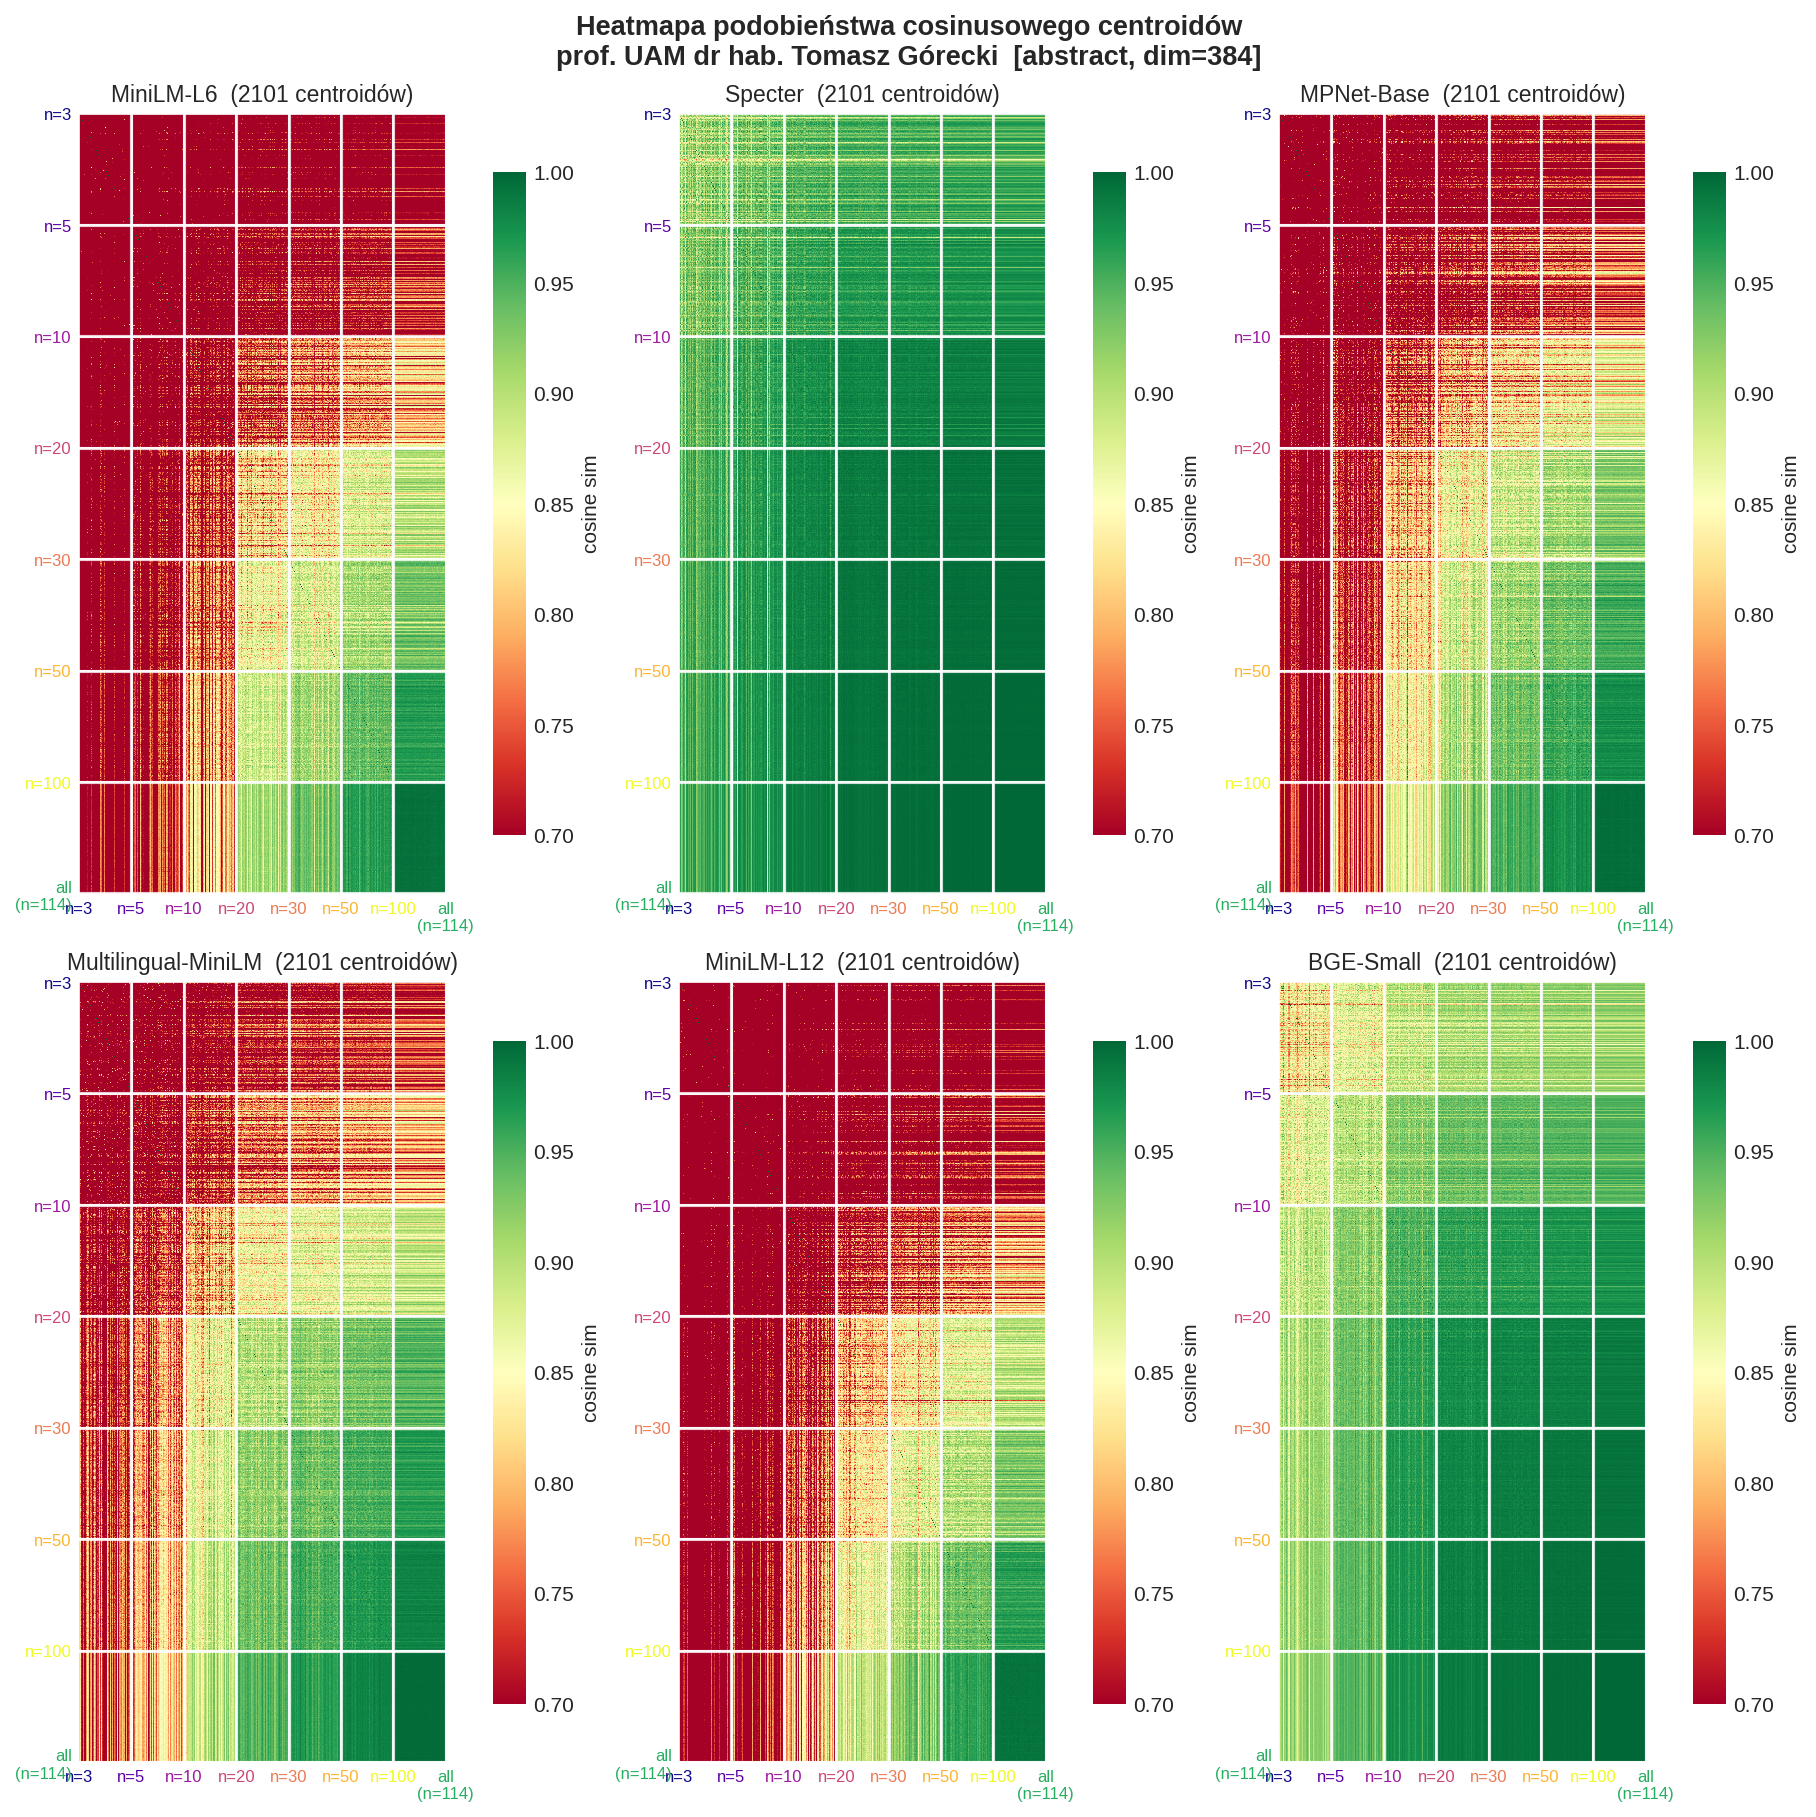
\includegraphics[width=\textwidth]{pubs_num_stability/heatmap_dense_stability.png}
    \caption{Heatmapa podobieństwa cosinusowego 2\,101~centroidów prof.~Góreckiego
    (eksperyment gęstego próbkowania).
    Oś posortowana wg rosnącego $k$; białe linie oddzielają grupy.
    Zielone bloki na~przekątnej dla Spectera i~BGE-Small wskazują,
    że~centroidy w~obrębie jednej grupy są do siebie bardzo podobne
    nawet przy małym~$k$.}
    \label{fig:heatmap_dense}
\end{figure}

Rysunek~\ref{fig:pca_dense} uwidacznia wyraźnie wzorzec konwergencji:
dla \textbf{Spectera} i~\textbf{BGE-Small} chmury wszystkich rozmiarów
są skupione blisko centroidu pełnego, a~różnica między $k=3$ a~$k=100$
jest minimalna.
Dla modeli ogólnych chmura przy $k=3$ jest bardzo szeroka i~obejmuje obszary
odległe od~gwiazdki -- dopiero przy $k \geq 30$ chmura wyraźnie się zawęża.

Tabela~\ref{tab:gorecki} przedstawia średnie podobieństwo cosinusowe
centroidu zbudowanego z~$k$~prac do centroidu pełnego
(300~próbek na~rozmiar, wszystkie sześć modeli).

\begin{table}[H]
\centering
\caption{Średnie podobieństwo cosinusowe
$\mathrm{sim}(\mathbf{c}_k,\,\mathbf{c}_\text{all})$
-- prof.~Górecki (114~prac), 300~losowych podzbiorów na~rozmiar.}
\label{tab:gorecki}
\begin{tabular}{r|cc|cccc}
\toprule
\textbf{$k$} &
\textbf{Specter} & \textbf{BGE-Small} &
\textbf{Multilingal-} & \textbf{MPNet-} & \textbf{MiniLM-} & \textbf{MiniLM-} \\
& & & \textbf{MiniLM} & \textbf{Base} & \textbf{L6} & \textbf{L12} \\
\midrule
  3  & 0{,}9129 & 0{,}9075 & 0{,}6290 & 0{,}5698 & 0{,}5304 & 0{,}5290 \\
  5  & 0{,}9427 & 0{,}9420 & 0{,}7352 & 0{,}6698 & 0{,}6441 & 0{,}6422 \\
 10  & 0{,}9729 & 0{,}9720 & 0{,}8387 & 0{,}8051 & 0{,}7670 & 0{,}7717 \\
 20  & 0{,}9872 & 0{,}9868 & 0{,}9194 & 0{,}8953 & 0{,}8738 & 0{,}8761 \\
 30  & 0{,}9922 & 0{,}9921 & 0{,}9494 & 0{,}9348 & 0{,}9154 & 0{,}9209 \\
 50  & 0{,}9965 & 0{,}9964 & 0{,}9759 & 0{,}9685 & 0{,}9608 & 0{,}9609 \\
100  & 0{,}9996 & 0{,}9996 & 0{,}9973 & 0{,}9964 & 0{,}9956 & 0{,}9956 \\
\bottomrule
\end{tabular}
\end{table}

\subsubsection{Eksperyment zbiorczy -- 107 naukowców UAM}

\begin{figure}[H]
    \centering
    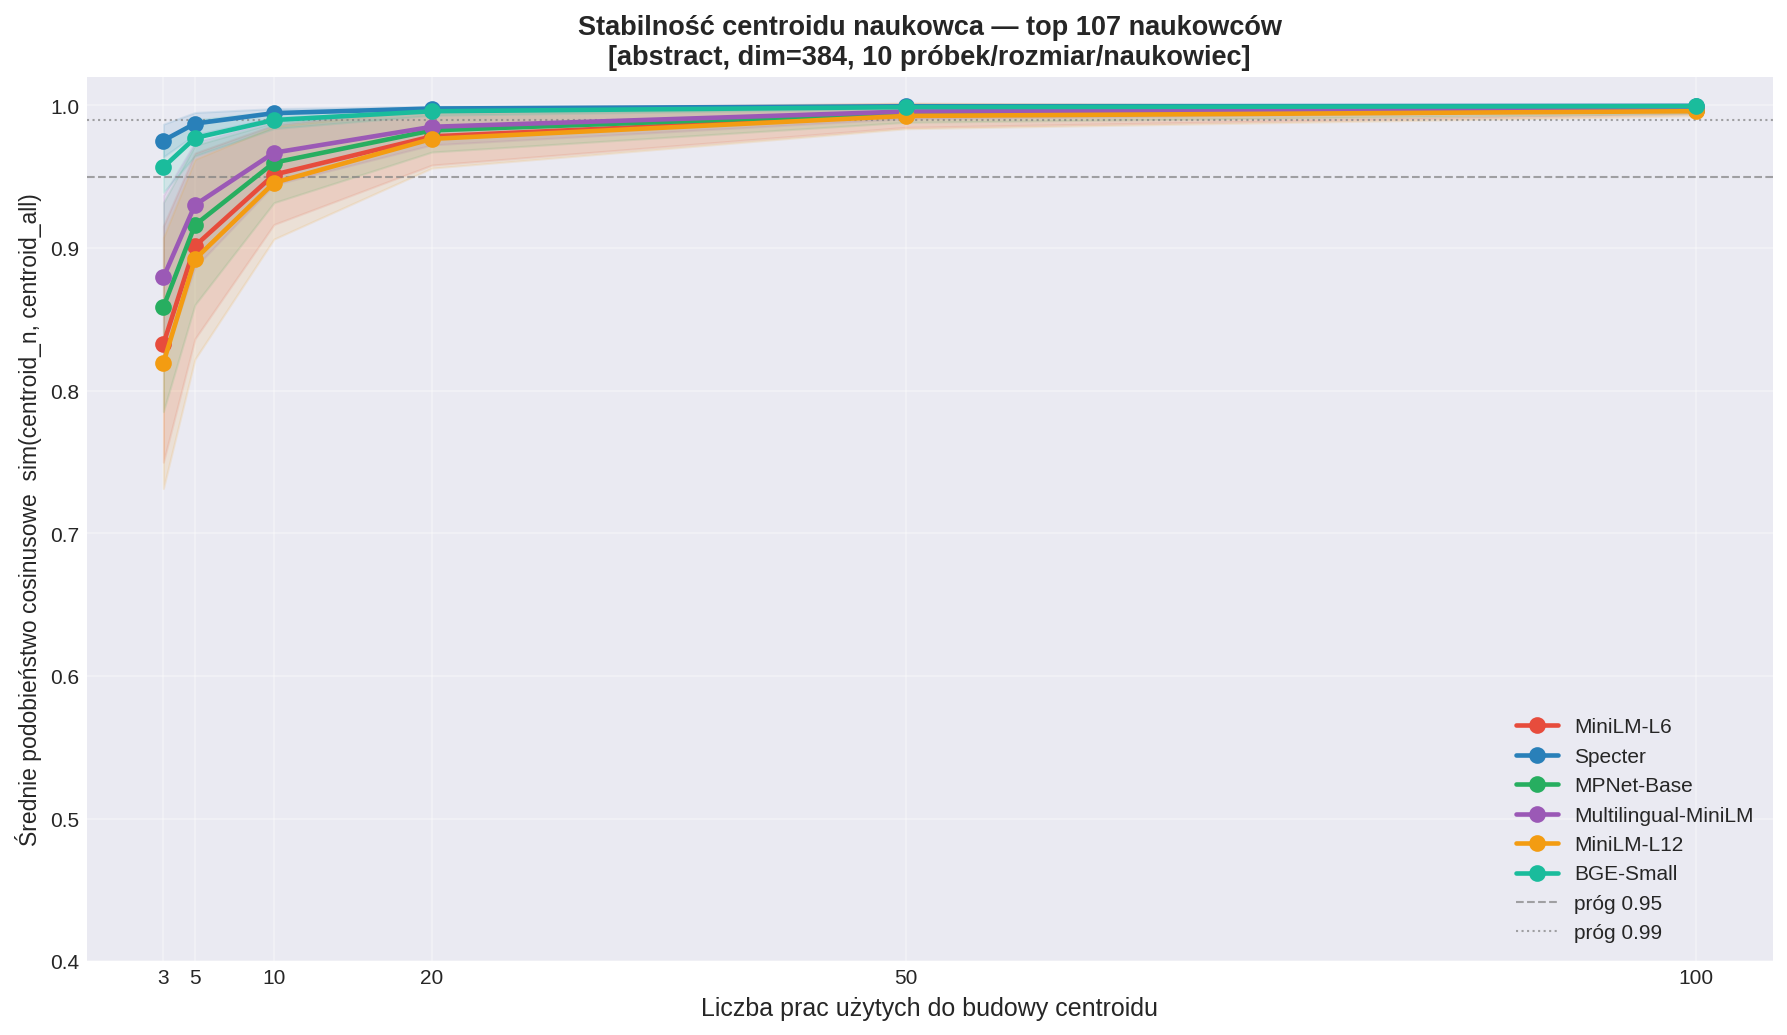
\includegraphics[width=\textwidth]{pubs_num_stability/stability_top_scientists.png}
    \caption{Średnie podobieństwo cosinusowe centroidu próbki do centroidu pełnego
    w~zależności od~liczby prac, uśrednione po~107~naukowcach UAM.
    Każda linia odpowiada innemu modelowi; pasmo ±1~odchylenie standardowe
    ilustruje zmienność między naukowcami.
    Przerywana linia pozioma~-- próg 0{,}95; kropkowana~-- próg 0{,}99.}
    \label{fig:stability_top}
\end{figure}

\begin{table}[H]
\centering
\caption{Średnie podobieństwo cosinusowe $\mathrm{sim}(\mathbf{c}_k,\mathbf{c}_\text{all})$
uśrednione po~naukowcach (eksperyment zbiorczy, 10~losowych podzbiorów/rozmiar/naukowiec).
Kolumna ,,Licz.\ nauk.''\ podaje liczbę naukowców uwzględnionych przy danym~$k$
(naukowcy z~dorobkiem $< k$ są pomijani).}
\label{tab:top_scientists}
\begin{tabular}{r|c|cc|cccc}
\toprule
\textbf{$k$} & \textbf{Licz.} &
\textbf{Specter} & \textbf{BGE-Small} &
\textbf{Multilin.-} & \textbf{MPNet-} & \textbf{MiniLM-} & \textbf{MiniLM-} \\
& \textbf{nauk.} & & & \textbf{MiniLM} & \textbf{Base} & \textbf{L6} & \textbf{L12} \\
\midrule
  3  & 107 & 0{,}9571 & 0{,}9523 & 0{,}8539 & 0{,}8090 & 0{,}7958 & 0{,}7854 \\
  5  & 106 & 0{,}9765 & 0{,}9747 & 0{,}9105 & 0{,}8813 & 0{,}8736 & 0{,}8667 \\
 10  &  88 & 0{,}9898 & 0{,}9885 & 0{,}9567 & 0{,}9412 & 0{,}9350 & 0{,}9294 \\
 20  &  55 & 0{,}9959 & 0{,}9954 & 0{,}9805 & 0{,}9725 & 0{,}9701 & 0{,}9691 \\
 50  &  20 & 0{,}9989 & 0{,}9987 & 0{,}9941 & 0{,}9914 & 0{,}9901 & 0{,}9898 \\
100  &   6 & 0{,}9995 & 0{,}9994 & 0{,}9970 & 0{,}9955 & 0{,}9951 & 0{,}9949 \\
\bottomrule
\end{tabular}
\end{table}

% ----------------------------------------------------------
\subsection{Dyskusja}
% ----------------------------------------------------------

\subsubsection{Dwie klasy modeli}

Wyniki ujawniają wyraźny podział sześciu modeli na~dwie klasy:

\paragraph{Klasa~I -- modele stabilne: Specter i~BGE-Small.}
Oba modele osiągają $\mathrm{sim} > 0{,}95$ już przy~$k = 5$~pracach
(agregat po~107~naukowcach: Specter~$0{,}976$, BGE-Small~$0{,}975$).
Przy $k = 10$ przekraczają próg~$0{,}98$.
Rozrzut odchylenia standardowego w~Exp3 jest wyraźnie mniejszy niż
dla modeli ogólnych, co~świadczy o~jednorodnym zachowaniu
niezależnie od~tego, którego naukowca reprezentujemy.

\paragraph{Klasa~II -- modele wrażliwe: MiniLM-L6, MiniLM-L12, MPNet-Base, Multilingual-MiniLM.}
Przy zaledwie 3~pracach modele te~osiągają jedynie
$0{,}53$--$0{,}63$ (Górecki) lub $0{,}79$--$0{,}85$ (agregat).
Wzrost podobieństwa jest jednak szybki -- przy~$k = 50$
wszystkie cztery modele przekraczają~$0{,}99$ w~eksperymencie zbiorczym,
a~przy~$k = 100$ zbiegają do~wartości porównywalnych z~klasą~I.

\subsubsection{Przyczyny różnic między modelami}

\textbf{Specter} został wytrenowany na~artykułach naukowych
z~sygnałem cytowań (podobne prace cytują się nawzajem)~\cite{specter2020}.
Taka procedura uczenia faworyzuje reprezentacje skupione tematycznie:
prace jednego naukowca lądują w~relatywnie wąskim obszarze przestrzeni,
dlatego centroid stabilizuje się szybko nawet przy małej próbce.

\textbf{BGE-Small} to~model wytrenowany metodą uczenia kontrastywnego
z~trudnymi negatywami (hard negative mining)~\cite{bge2023},
co~sprawia, że~embeddingi są zwarte i~zorientowane tematycznie.
Model ten generuje bardzo skupione reprezentacje dokumentów
z~tej samej dziedziny -- stąd jego wysoka stabilność.

Modele ogólne (MiniLM, MPNet) są optymalizowane na~szerokich
zbiorach zdań z~różnych domen.
Reprezentują one bardziej ,,płaską'' przestrzeń, w~której prace
z~tego samego naukowca mogą być rozrzucone szerzej --
szczególnie gdy naukowiec publikuje w~kilku różnych dziedzinach.
Ilustruje to~przypadek prof.~Góreckiego, którego prace dotyczą
zarówno statystyki funkcjonalnej, jak i~klasyfikacji szeregów
czasowych i~chemometrii żywności.

\subsubsection{Różnica między eksperymentem pilotażowym a~zbiorczym}

Wartości podobieństwa w~Exp3 (agregat) są systematycznie wyższe
niż w~Exp2 dla samego Góreckiego
(np.\ MiniLM-L6, $k=3$: $0{,}530$ vs.\ $0{,}796$).
Wynikają z~tego dwa wnioski.
Po~pierwsze, Górecki ma wyjątkowo szeroki interdyscyplinarny profil,
co~czyni go~trudniejszym przypadkiem niż przeciętny naukowiec.
Po~drugie, przy uśrednianiu po~107~naukowcach część badaczy ma
bardzo skoncentrowane profile (np.\ wąskie specjalności),
co~podnosi średnią.
Oba fakty oznaczają, że~podane progi należy traktować jako
\textbf{oszacowania konserwatywne}: dla typowego naukowca
z~jednorodnym profilem stabilizacja nastąpi szybciej.

\subsubsection{Praktyczne zalecenia dla systemu rekomendacji}

Na~podstawie obu eksperymentów formułujemy następujące wnioski praktyczne:

\begin{itemize}
    \item \textbf{Specter i~BGE-Small} zapewniają stabilny profil już
    przy~\textbf{$k \approx 10$ pracach} ($\mathrm{sim} > 0{,}98$).
    Modele te są zalecanym wyborem, gdy baza danych zawiera naukowców
    z~małym dorobkiem.

    \item \textbf{Modele ogólne} wymagają~\textbf{$k \approx 30$--$50$ prac}
    dla uzyskania $\mathrm{sim} > 0{,}95$.
    Są dobrym wyborem dla naukowców z~bogatym dorobkiem,
    ale~profil naukowców z~mniej niż 20~pracami może być niestabilny.

    \item Dla naukowców z~\textbf{ponad 50~pracami} różnice między modelami
    stają się znikome (wszystkie przekraczają $\mathrm{sim} > 0{,}99$).

    \item Wynik ten sugeruje, że~\textbf{liczba prac jest osobnym wymiarem
    jakości profilu}, niezależnym od~wyboru modelu.
    System rekomendacji powinien informować użytkownika,
    ile prac danego naukowca zostało uwzględnionych w~jego profilu,
    a~ewentualnie przypisywać niższy ,,współczynnik zaufania''
    profilom opartym na~małej liczbie publikacji.
\end{itemize}

% ----------------------------------------------------------
\subsection{Podsumowanie}
% ----------------------------------------------------------

Przeprowadzone eksperymenty wykazały, że~stabilność centroidu profilu naukowca
silnie zależy od~wyboru modelu embeddingowego.
Modele Specter i~BGE-Small -- wytrenowane odpowiednio na~literaturze naukowej
i~za pomocą uczenia kontrastywnego -- tworzą kompaktowe, tematycznie skupione
reprezentacje, dzięki czemu centroid stabilizuje się przy zaledwie 10~pracach.
Modele ogólnego przeznaczenia osiągają porównywalną stabilność dopiero
przy~$\sim$50~pracach.
Wyniki te mają bezpośrednie przełożenie na~decyzję o~wyborze modelu
w~systemie rekomendacji dla środowisk akademickich,
gdzie część naukowców -- zwłaszcza doktoranci i~asystenci --
dysponuje stosunkowo skromnym dorobkiem.

% ============================================================
%  BIBLIOGRAFIA (jeśli używasz bibtex, dodaj do swojego .bib):
% ============================================================
%
%  @inproceedings{specter2020,
%    title   = {{SPECTER}: Document-level Representation Learning
%               using Citation-informed Transformers},
%    author  = {Cohan, Arman and Feldman, Sergey and Beltagy, Iz
%               and Downey, Doug and Weld, Daniel S.},
%    booktitle = {ACL},
%    year    = {2020}
%  }
%
%  @article{bge2023,
%    title   = {{C-Pack}: Packaged Resources To Advance General
%               Chinese Embedding},
%    author  = {Zhang, Peitian and others},
%    journal = {arXiv:2309.07597},
%    year    = {2023}
%  }
%
%  @article{johnson1984extensions,
%    title   = {Extensions of {Lipschitz} mappings into a {Hilbert} space},
%    author  = {Johnson, William B. and Lindenstrauss, Joram},
%    journal = {Contemporary Mathematics},
%    volume  = {26},
%    pages   = {189--206},
%    year    = {1984}
%  }


\subsection{Interdyscyplinarność naukowca}
\label{subsec:interdisciplinarity}

Eksperymenty pilotażowe przeprowadzono na~prof.~UAM dr~hab.~Tomaszu
Górecki -- badaczu o~wyjątkowo szerokim i~interdyscyplinarnym dorobku,
obejmującym statystykę funkcjonalną, klasyfikację szeregów czasowych
i~chemometrię żywności.
Wyniki dla tego naukowca są systematycznie \textbf{gorsze} niż wyniki
uśrednione po~107~badaczach (np.\ MiniLM-L6, $k=3$: $0{,}530$
dla Góreckiego vs. $0{,}796$ w~agregacie).

Zjawisko to~wyjaśnia geometria przestrzeni embeddingów:
naukowiec interdyscyplinarny publikuje prace z~różnych dziedzin,
których wektory są rozrzucone w~różnych regionach przestrzeni.
Centroid z~małej próbki losowych prac może trafić
w~obszar reprezentatywny tylko dla jednej z~dziedzin,
dając niepełny obraz całego profilu.
Naukowiec o~wąskiej, jednorodnej specjalizacji ma~prace skupione
w~małym regionie przestrzeni -- losowa próbka kilku prac
daje centroid bliski centroidowi pełnemu.

\textbf{Wniosek:} Interdyscyplinarność jest czynnikiem niezależnym
od~liczby prac -- nawet naukowiec z~dużym, interdyscyplinarnym
dorobkiem może wymagać wielu prac do~uformowania stabilnego profilu.
System rekomendacji powinien ideowo uwzględniać tę~właściwość,
np.\ poprzez reprezentację multimodalną (kilka centroidów
per naukowiec, jeden dla każdej dziedziny).

% ----------------------------------------------------------
\section{Dyskusja i~wnioski}
\label{sec:discussion}
% ----------------------------------------------------------

Eksperymenty opisane w~niniejszym rozdziale dostarczyły odpowiedzi
na~trzy główne pytania badawcze:

\paragraph{1.~Czy podejście embeddingowe w~ogóle działa?}

Tak -- z~dużym marginesem pewności.
Obydwa testowane modele (SPECTER i~MiniLM-L6) osiągają
statystycznie wysoce istotną separację współautorów od~losowych par
($p < 10^{-16}$, $d > 1{,}5$) bez~żadnego ręcznego nadzoru tematycznego.
Podejście oparte wyłącznie na~tekście publikacji jest zatem
solidnym punktem wyjścia dla systemu rekomendacji.

\paragraph{2.~Który model wybrać?}

Odpowiedź zależy od~liczby dostępnych publikacji:
\begin{itemize}
    \item Jeśli baza zawiera wielu naukowców z~\textbf{małym dorobkiem
    ($< 20$~prac)}: należy zastosować \textbf{SPECTER lub~BGE-Small},
    które osiągają stabilność ($\mathrm{sim} > 0{,}95$)
    już przy~$k = 5$~pracach.
    \item Jeśli zdecydowana większość naukowców ma
    \textbf{ponad 30~prac}: modele z~rodziny \textbf{MiniLM lub~MPNet}
    są akceptowalnym wyborem i~generują spójniejsze rankingi
    (Jaccard $\approx 0{,}79$ wewnątrz rodziny).
    \item Przy \textbf{ponad 50~pracach} różnice między wszystkimi
    modelami zanikają.
\end{itemize}
Model Multilingual-MiniLM nie~był najlepszy w~żadnej kategorii
i~wykazywał największe rozbieżności z~pozostałymi modelami --
jego użycie należy ograniczyć do~scenariuszy z~wielojęzycznym
korpusem publikacji.

\paragraph{3.~Czy abstrakt jest lepszy niż tytuł?}

Abstrakty wnoszą semantycznie spójną informację uzupełniającą
(spójne przesunięcia w~PCA, Jaccard $\approx 0{,}70$
dla tego samego modelu, różne typy tekstu).
W~praktyce warto stosować abstrakty, gdy~są dostępne,
przy~świadomości, że~część publikacji (szczególnie starszych)
może ich nie~posiadać.
Podejście hybrydyczne -- abstrakt gdy~dostępny, tytuł gdy~nie --
jest rozsądnym kompromisem.

\paragraph{Ograniczenia.}

Głównym ograniczeniem ewaluacji jest użycie współautorstwa
jako proxy dla podobieństwa naukowego.
Naukowcy mogą być współautorami z~powodów administracyjnych
lub projektowych, a~brak współautorstwa nie~oznacza braku
zbieżności zainteresowań.
Brak złotego standardu (ręcznych ocen eksperckich)
uniemożliwia ostateczne rozstrzygnięcie, który model wskazuje
``właściwych'' kandydatów do~rekomendacji.
Kolejnym ograniczeniem jest jednorodność instytucjonalna danych:
zbiór pochodzi z~jednego wydziału jednej uczelni,
co~może nie~odzwierciedlać zachowania modeli na~bardziej
zróżnicowanych populacjach.

% ----------------------------------------------------------
\section{Dalsze kierunki badań}
\label{sec:future_work}
% ----------------------------------------------------------

Na~podstawie przeprowadzonych eksperymentów wskazujemy
następujące kierunki dalszych prac:

\begin{enumerate}
    \item \textbf{Ewaluacja ekspercka.}
    Kluczowym uzupełnieniem byłoby przeprowadzenie ankiety
    wśród samych naukowców WMIi, weryfikującej trafność
    rekomendowanych par. Taka ocena pozwoliłaby odejść
    od~pośredniego proxy współautorstwa i~bezpośrednio zmierzyć
    użyteczność systemu dla końcowego użytkownika.

    \item \textbf{Fine-tuning modeli na~danych UAM.}
    Dostrojenie modelu (np.\ SPECTER lub~MiniLM)
    na~parach prac naukowców z~WMIi -- z~sygnałem z~grafu
    współautorstwa lub~cytowań -- mogłoby znacząco poprawić
    jakość profilowania dla tej specyficznej populacji.

    \item \textbf{Reprezentacja multimodalna dla naukowców interdyscyplinarnych.}
    Zamiast jednego centroidu można reprezentować profil
    naukowca jako \emph{zbiór centroidów} (po~jednym na~klaster tematyczny),
    wyznaczonych np.\ algorytmem $k$-means na~embeddingach jego prac.
    Taka reprezentacja mogłaby lepiej uchwycić wielowymiarowość
    zainteresowań naukowych.

    \item \textbf{Ocena konkatenacji embeddingów.}
    Eksperyment z~konkatenacją (sekcja~\ref{subsec:concat})
    miał charakter eksploracyjny.
    Pełna ewaluacja -- z~porównaniem do~najlepszego
    pojedynczego modelu na~tym samym zadaniu walidacyjnym --
    jest niezbędna, by~ocenić rzeczywisty zysk z~tej metody.

    \item \textbf{Integracja z~grafem cytowań.}
    Uzupełnienie profilu tekstowego o~reprezentację
    naukowca w~grafie cytowań (np.\ metodą GraphSAGE)
    mogłoby uchwycić wymiar ``wpływu naukowego'',
    niewidoczny w~samym tekście publikacji.

    \item \textbf{Modele specjalizowane dla poddziedzin.}
    Testowane modele traktują całą matematykę i~informatykę
    jako jedną domenę. Modele specjalizowane dla wąskich
    dziedzin (np.\ \texttt{math-bert}, \texttt{cs-bert})
    mogłyby poprawić rozdzielczość profilowania
    w~obrębie jednej dyscypliny.
\end{enumerate}

% ============================================================
%  BIBLIOGRAFIA — dodaj do swojego .bib:
% ============================================================
%
% @inproceedings{specter2020,
%   title   = {{SPECTER}: Document-level Representation Learning
%              using Citation-informed Transformers},
%   author  = {Cohan, Arman and Feldman, Sergey and Beltagy, Iz
%              and Downey, Doug and Weld, Daniel S.},
%   booktitle = {Proceedings of ACL},
%   year    = {2020}
% }
%
% @inproceedings{scibert2019,
%   title   = {{SciBERT}: A Pretrained Language Model for Scientific Text},
%   author  = {Beltagy, Iz and Lo, Kyle and Cohan, Arman},
%   booktitle = {Proceedings of EMNLP},
%   year    = {2019}
% }
%
% @article{bge2023,
%   title   = {{C-Pack}: Packaged Resources to Advance General
%              Chinese Embedding},
%   author  = {Zhang, Peitian and others},
%   journal = {arXiv:2309.07597},
%   year    = {2023}
% }
%
% @inproceedings{sbert2019,
%   title   = {Sentence-{BERT}: Sentence Embeddings using
%              Siamese {BERT}-Networks},
%   author  = {Reimers, Nils and Gurevych, Iryna},
%   booktitle = {Proceedings of EMNLP},
%   year    = {2019}
% }
%
% @inproceedings{wang2020minilm,
%   title   = {{MiniLM}: Deep Self-Attention Distillation for
%              Task-Agnostic Compression of Pre-Trained Transformers},
%   author  = {Wang, Wenhui and Wei, Furu and Dong, Li and
%              Bao, Hangbo and Yang, Nan and Zhou, Ming},
%   booktitle = {NeurIPS},
%   year    = {2020}
% }
%
% @inproceedings{mpnet2020,
%   title   = {{MPNet}: Masked and Permuted Pre-training for
%              Language Understanding},
%   author  = {Song, Kaitao and Tan, Xu and Qin, Tao and
%              Lu, Jian and Liu, Tie-Yan},
%   booktitle = {NeurIPS},
%   year    = {2020}
% }
%
% @article{priem2022openalex,
%   title   = {{OpenAlex}: A fully-open index of scholarly works,
%              authors, venues, institutions, and concepts},
%   author  = {Priem, Jason and Piwowar, Heather and Orr, Richard},
%   journal = {arXiv:2205.01833},
%   year    = {2022}
% }
%
% @article{jl1984,
%   title   = {Extensions of {Lipschitz} mappings into a {Hilbert} space},
%   author  = {Johnson, William B. and Lindenstrauss, Joram},
%   journal = {Contemporary Mathematics},
%   volume  = {26},
%   pages   = {189--206},
%   year    = {1984}
% }
%
% @book{cohen1988,
%   title   = {Statistical Power Analysis for the Behavioral Sciences},
%   author  = {Cohen, Jacob},
%   edition = {2nd},
%   publisher = {Lawrence Erlbaum Associates},
%   year    = {1988}
% }
%
% @techreport{ic_report,
%   title   = {Embeddingi Autorów dla Systemu Rekomendacji Naukowców:
%              Porównanie Modeli {SPECTER} i {MiniLM}},
%   author  = {Paszke, Jakub and Rolewski, Miłosz},
%   institution = {Wydział Matematyki i Informatyki UAM},
%   year    = {2024}
% }
